%\chapter{Thermomechanics}
%\textit{by Wenqing Wang, Norihiro Watanabe and J�rgen Hesser}

%makro
%\providecommand{\sembrack}[1]{[\![#1]\!]}
\providecommand{\pD}[2]{\dfrac{\partial #1}{\partial #2}}
\providecommand{\oD}[2]{\dfrac{\mathrm d #1}{\mathrm d  #2}}
\providecommand{\abs}[1]{\lvert #1 \rvert}
%%\providecommand{\abs}[1]{\left\lvert #1 \right\rvert}
\providecommand{\norm}[1]{\left\lVert #1 \right\rVert}

\newcommand{\od}{\mathrm d}
%%%
\newcommand{\js}{\mathscr S}
%%%
%%material index
\newcommand{\pl}{\scriptscriptstyle \mathrm p}
\newcommand{\el}{\scriptscriptstyle \mathrm e}

%%Geometry
\newcommand{\Point}{ \bm x}

%%Displacement field
\newcommand{\Pressure}{p}
\newcommand{\Stress}{ \bm \sigma}
\newcommand{\inPStress}{ \Stress_{\imath}} %%% in-plane stress
\newcommand{\stress}{ \sigma}
\newcommand{\devStrs}{\bm s}
\newcommand{\Strain}{ \bm \epsilon}
\newcommand{\strain}{ \epsilon}
\newcommand{\Disp}{\mathbf u}
\newcommand{\disp}{u}
\newcommand{\vel}{\bf v}
\newcommand{\per}{\mathbf k}
\newcommand{\grv}{\mathbf g}
%%Plasticity
\newcommand{\yld}{ f}
\newcommand{\ppo}{ g}
\newcommand{\pHard}{\mathcal H}
\newcommand{\CT}{\mathbb C}
\newcommand{\DT}{\mathbb D}
\newcommand{\EM}{{\bm C}^{\el}}
\newcommand{\PM}{{\bm C}^{\pl}}
\newcommand{\EPM}{{\bm C}^{\el\pl}}
\newcommand{\mEM}{{\bm D}^{\el}}
\newcommand{\mPM}{{\bm D}^{\pl}}
\newcommand{\mEPM}{{\bm D}^{\el\pl}}
\newcommand{\rdl}{\dot \lambda}
\newcommand{\dl}{\lambda}
\newcommand{\dens}{\rho}

%%Flow
\newcommand{\densc}{\dens^{\gamma}}
\newcommand{\presc}{p^{\gamma}}
\newcommand{\pres}{p}
\newcommand{\sat}{S}
\newcommand{\Satc}{S^{\gamma}}
\newcommand{\RelK}{k^{\gamma}_{rel}}
\newcommand{\RelKa}{k_{rel}}
\newcommand{\poro}{n}
\newcommand{\Fluxf}{\mathbf{q}_{\scriptscriptstyle f}}
\newcommand{\Fluxv}{\mathbf{q}_{\scriptscriptstyle v}}
\providecommand{\perm}{ \mathbf k}
\newcommand{\asup}[2]{#1^#2}
\newcommand{\asub}[2]{#1_#2}
\newcommand{\supsub}[3]{{#1}^{#2}_{#3}}
\newcommand{\FlxDf}{\mathbf{J}}
\newcommand{\Sat}{S}
%%Heat
\newcommand{\HC}{C_p}
\newcommand{\Flux}{\mathbf{q}}

%%%FEM
\newcommand{\test}{w}
\newcommand{\Test}{\bm w}
\newcommand{\TestS}{\mathcal V}
\newcommand{\sh}{N}
% \newcommand{\Sh}{{\bm N}}

%%Math
\newcommand{\intD}{{\int}_{\Omega}}
\newcommand{\intB}{{\int}_{\Gamma}}
\newcommand{\dDom}{\,\mathrm{d} \Omega}
\newcommand{\dBdry}{\,\mathrm{d} \Gamma}
\newcommand{\nrl}{\mathbf n}
\newcommand{\tgl}{\mathbf t}
\newcommand{\I}{\mathbf I}

\newcommand {\StrainT}{ \bm \epsilon}

In this chapter, we consider coupled thermo-mechanical (TM) processes in a porous medium. 
%
%-----------------------------------------------------------
%\section{Theory}
%\subsection*{Heat transport in solids or porous media}
%\label{ssec:heat}
For heat transport problem in any medium, the governing equation is given by
\begin{gather}
 \dens \HC T' = -\nabla \Flux_{\mbox{\tiny T}}+ Q_{\mbox{\tiny T}}(\bm x, t), \,\bm x\in \mathbb R^3
 \label{eq:Tgvn}
\end{gather}
where $\dens$ is medium density, $\HC(T)$ is the specific heat capacity, $ Q_{\mbox{\tiny T}}$ is heat source and  $\Flux_{\mbox{\tiny T}}$ is the heat flux,
which takes
the forms
\begin{equation}
 \Flux_{\mbox{\tiny T}} = -K_e\nabla, T
 \label{eq:tfluxs}
\end{equation}
for solid and
\begin{equation}
 \Flux_{\mbox{\tiny T}} = -K_e\nabla\,T+\poro\sum_{\gamma}^{phase}(\densc\HC^{\gamma}) T \vel, \,\gamma=\mbox{liquid, gaseous }
 \label{eq:tflux1}
\end{equation}
for porous media considering of advective and diffusive fluxes  with $K_e$ the heat conductivity.
For porous  media, the specific heat capacity consists of
 portions of solid, liquid and gaseous phase as
\begin{equation}
  \dens \HC = \sum_{\gamma}^{phase}(\densc\HC^{\gamma})
 \label{eq:tcp}
\end{equation}
where $\gamma$ specifies solid, liquid or  gaseous phase. The  boundary conditions are given by
\begin{equation}
 \Flux_{\mbox{\tiny T}}\cdot\nrl=q^{\mbox{\tiny
 T}}_{\scriptscriptstyle{\Gamma}},\, \mbox{or}\quad
 T=T_{\scriptscriptstyle{\Gamma}}, \,
 \forall\, \Point\, \in \partial \Omega
 \label{eq:tbc1}
\end{equation}
and the initial condition reads
\begin{equation}
 T(\Point, t)=T_0(\Point), \, \forall\, \Point\, \in \Omega
 \label{eq:tini1}
\end{equation}
with $\nrl$, the normal direction at $\Point  \in \partial \Omega$

%\subsection*{Thermal stress}
For mechanical process, we consider the total strain rate $\Delta \StrainT$ can be admissible  decomposed into components such as reversible (elastic),
temperature deduced as
\begin{equation}
\Delta\StrainT=\CT(\Delta\StrainT^{e}-\alpha\,\I \Delta T)
 \label{eq:estrain}
\end{equation}
where $\CT$ is the constitutive tensor, $\alpha$ is the linear thermal expansion coefficient, $\I$ is the identity tensor, and $\Delta T$ is temperature change. With the generalized Hook's law, the total
stress with the thermal effect can be expressed as
\begin{equation}
\Delta\Stress=\CT(\Delta\StrainT-\alpha\,\I \Delta T)
 \label{eq:estress}
\end{equation}
with $\Stress$ is the stress tensor.
%
The volume of a solid is increasing or decreasing with temperature changes. Homogeneous bodies expand evenly in each direction by increasing temperatures. In this case no variation of the stresses occurs. If the deformation of the solid is prevented, the stresses are increasing or decreasing with temperature changes. %(Beitz et al., 1987). 
This phenomenon can be easily calculated by analytical solutions of the Hooke's linear elastic model. The equations of the mechanical behaviour base on the Hooke's law for linear elastic materials:
\begin{eqnarray}
\varepsilon_x & = & \frac{1}{E}\cdot
\left(
\sigma_x\,-\,\nu\cdot
\left(
\sigma_y\,+\,\sigma_z
\right)
\right)\,+\,\alpha\cdot\Delta T
\label{eq61} \\[1.5ex]
\varepsilon_y & = & \frac{1}{E}\cdot
\left(
\sigma_y\,-\,\nu\cdot
\left(
\sigma_x\,+\,\sigma_z
\right)
\right)\,+\,\alpha\cdot\Delta T
\label{eq62} \\[1.5ex]
\varepsilon_z & = & \frac{1}{E}\cdot
\left(
\sigma_z\,-\,\nu\cdot
\left(
\sigma_x\,+\,\sigma_y
\right)
\right)\,+\,\alpha\cdot\Delta T
\label{eq63}
\end{eqnarray}

\noindent
where  $\varepsilon_i$ are strains, $\sigma_i$ are stresses, $E$ is Young's modulus, and $\nu$ is Poisson's ratio. 

%{\small
%with
%\begin{itemize}
%\item[$\varepsilon_i$] -- strains
%\item[$\sigma_i$] -- stresses in Pa
%\item[$E$] -- Young's modulus in Pa
%\item[$\nu$] -- Poisson's ratio
%\item[$\alpha$] -- thermal expansion in K$^{-1}$
%\item[$\Delta T$] -- temperature change in K
%\end{itemize}
%
%indices:
%
%$x,\, y,\, z\;$	- $\;x,\, y,\, z$-direction.
%}


%-----------------------------------------------------------
%\section{Thermoelastic plate (2D)}
\label{sec:tm2d}
\subsection{Definition}
We consider a thermoelastic consolidation on a 2D vertical plate under plane strain conditions. All parameters are dimensionless. The domain has a rectangular shape with size of 10 $\times$ 10. Material properties are listed in Table \ref{tab:tm2D}. Initial condition is given by
\[
\mathbf \sigma_{0} = \mathbf 0, \, T_0=198.15
\]
and boundary conditions are depicted in Figure \ref{fig:TMbc}. Gravity force is considered in $y$ direction. 

\begin{table}[!htb]
\caption{Model parameters}
\label{tab:tm2D}
\centering
\begin{tabular}{llrr}
\toprule
Symbol & Parameter & Value & Unit \\
\midrule
$E$ & Young's modulus & $3 \cdot 10^{3}$  & $-$ \\
$\nu$ & Poisson's ratio & $0.3$       & $-$ \\
$\rho$ & Density    & $1.0$        & $-$ \\
$\beta$ & Volumetric thermal expansion & $1.0$         & $-$ \\
$c$ & Specific heat capacity & $1.0$         & $-$ \\
$\lambda$ & Thermal conductivity & $1.0$         & $-$ \\
\bottomrule
\end{tabular}
\end{table}

\begin{figure}[!htbp]
\centering
%\input{PART_III/TM/e1.eepic}
\epsfig{figure=PART_III/TM/figures/e1,height=5cm}
\caption{Boundary conditions for TM coupling plane strain problem }
\label{fig:TMbc}
\end{figure}

\subsection{Solution}
%\subsubsection{Analytical solution}
%\subsubsection{Numerical solution}
%%The results are compared with the analytic solution as well.
%All parameters are dimensionless. 
Numerical simulation is conducted with time step size 0.1. The simulation runs 100 steps. The domain is discretized into quadrilateral elements (Figure \ref{fig:TM2Mesh}). 

%\begin{figure}[!htb]
\begin{figure}[!htbp]
\centering
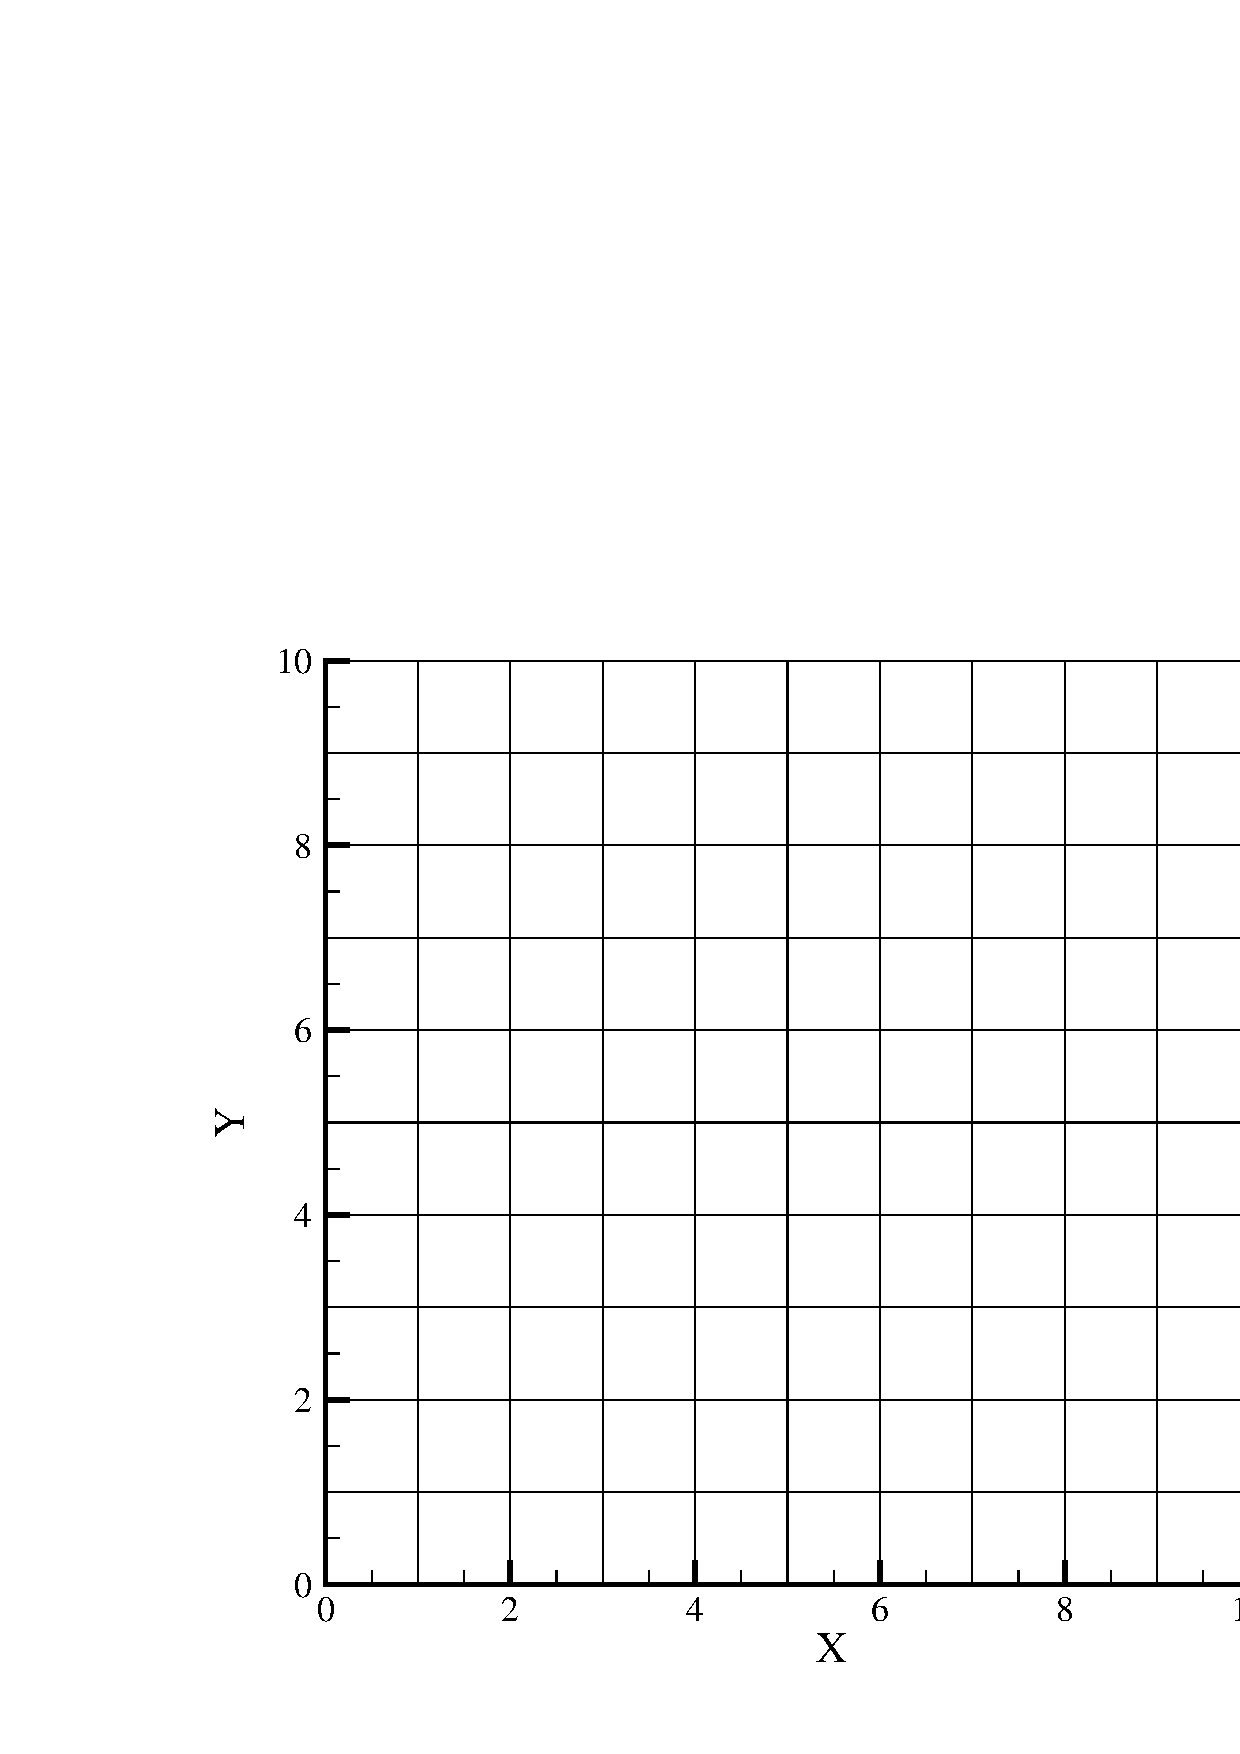
\includegraphics[height=5cm]{PART_III/TM/figures/2D_mesh}\\
\caption{Mesh for TM coupling plane strain problem }
\label{fig:TM2Mesh}
\end{figure}




\subsection{Results}
Fig. \ref{fig_TM1_r} provides the distribution of temperature and vertical stress after 100 time steps. The vertical stress distribution shows the effect of gravity force. The results of 2D model are compared with that of 3D model in the next example.

%\begin{figure}[!htb]
\begin{figure}[!htbp]
\begin{center}
\epsfig{figure=PART_III/TM/figures/2D_T,height=6cm}
\epsfig{figure=PART_III/TM/figures/2D_syy,height=6cm}
\end{center}
\caption{Distribution of temperature and vertical stress after 100 time steps}
\label{fig_TM1_r}
\end{figure}


%\clearpage
%\section{Thermoelastic cube (3D)}
\subsection{Definition}
The problem given in section \ref{sec:tm2d} for plane strain conditions is considered in a 3D model. 
Initial and boundary conditions are similar to that described in section \ref{sec:tm2d}.
Material properties are given in Table \ref{tab:tm2D}. 
Results of the 3D model are compared with that of the 2D model.

\subsection{Solution}
%\subsubsection{Analytical solution}
%\subsubsection{Numerical solution}
Numerical simulation is conducted with a 3D model obtained by extruding the 2D model in off-plane direction for 1 unit.
The domain is discretized into hexahedra (Figure \ref{fig:TM3Mesh}).

\begin{figure}[!htb]
\centering
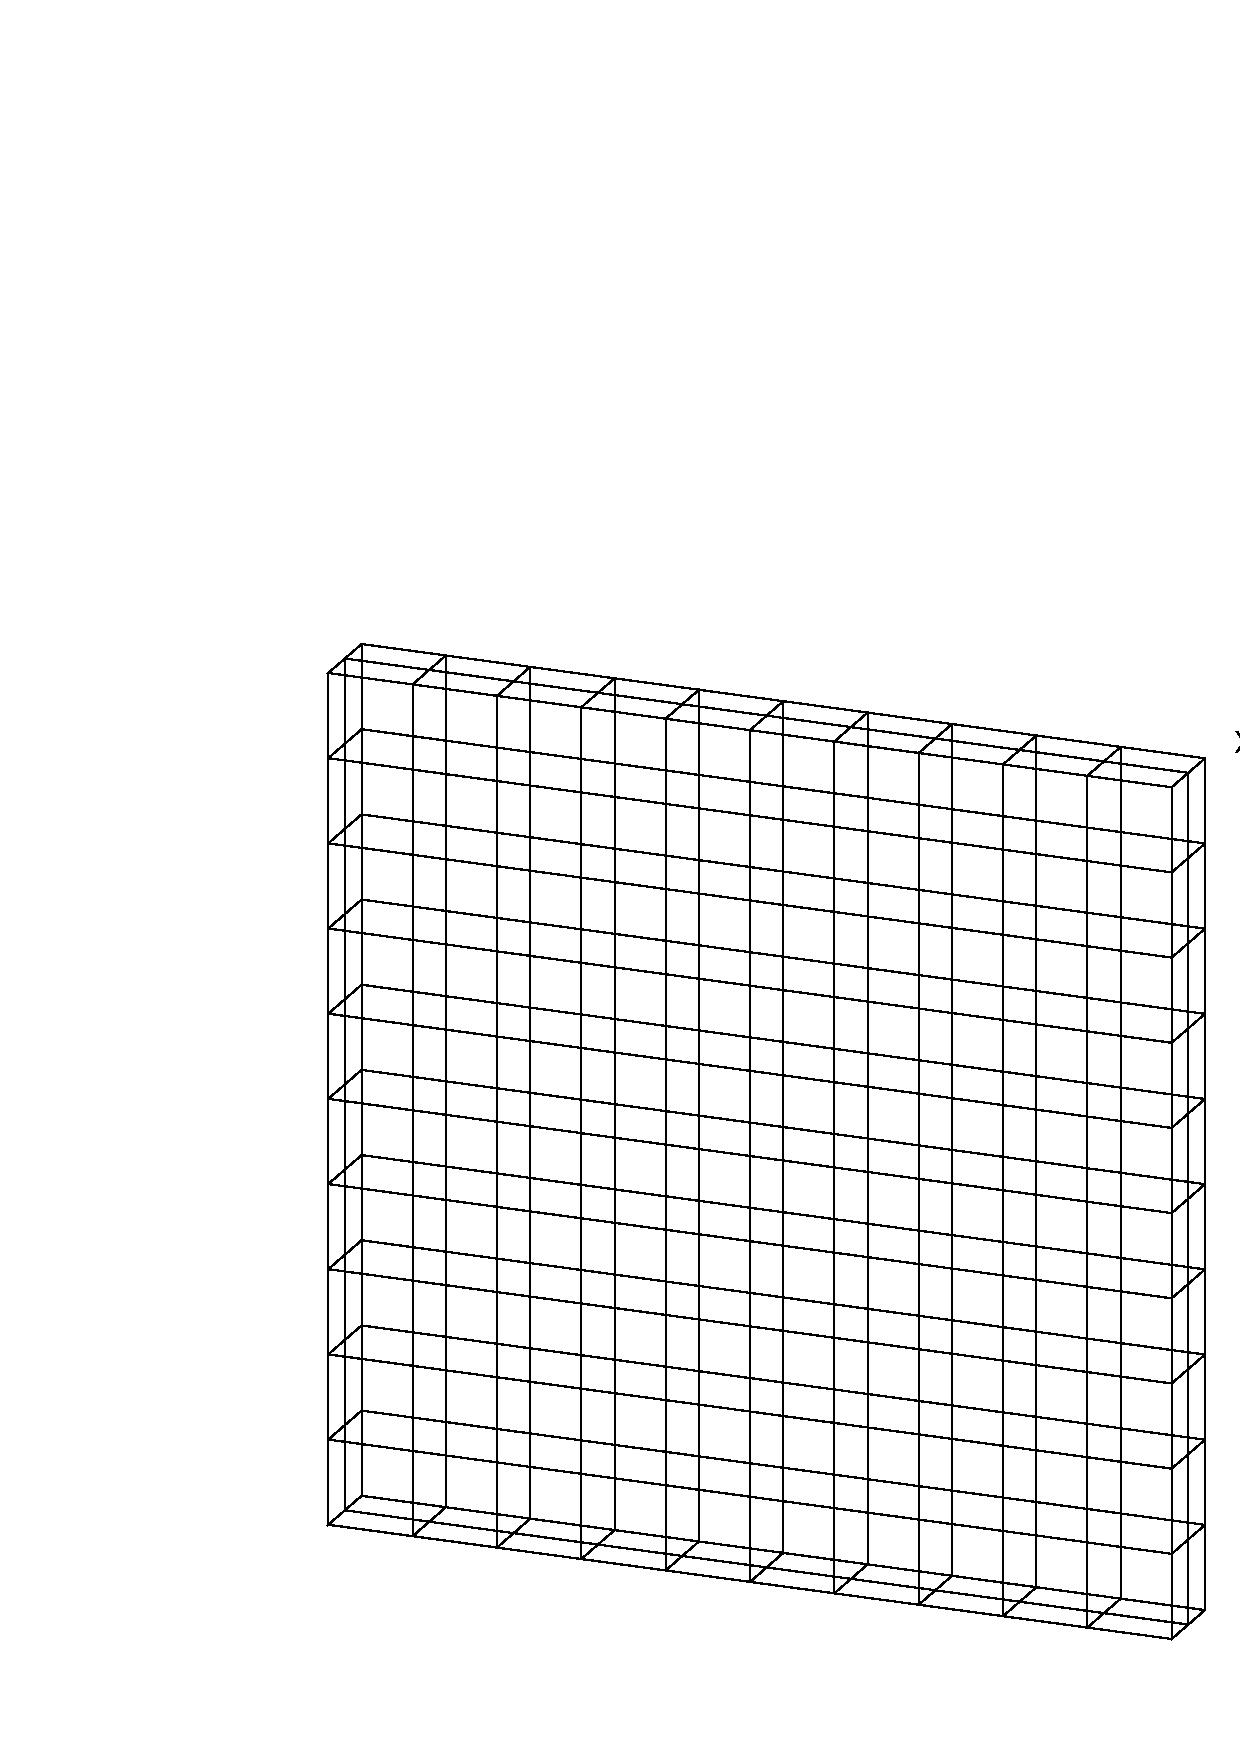
\includegraphics[height=5cm]{PART_III/TM/figures/3D_mesh}\\
\caption{Mesh for TM coupling 3D problem }
\label{fig:TM3Mesh}
\end{figure}



\subsection{Results}
Figure \ref{fig_TM2_r} provides the distribution of temperature and vertical stress after 100 time steps.
The distribution is identical to that given in Figure \ref{fig_TM1_r} for plane strain problem.
Figure \ref{fig:TMcmp} gives a comparison about the variation of state variables at the gravity center of 2D and 3D model.
 The results agree well with each other.

\begin{figure}[!htbp]
\begin{center}
\epsfig{figure=PART_III/TM/figures/3D_T,height=6cm}
\epsfig{figure=PART_III/TM/figures/3D_szz,height=6cm}
\end{center}
\caption{Distribution of temperature and vertical stress}
\label{fig_TM2_r}
\end{figure}

\begin{figure}[!htbp]
\centering
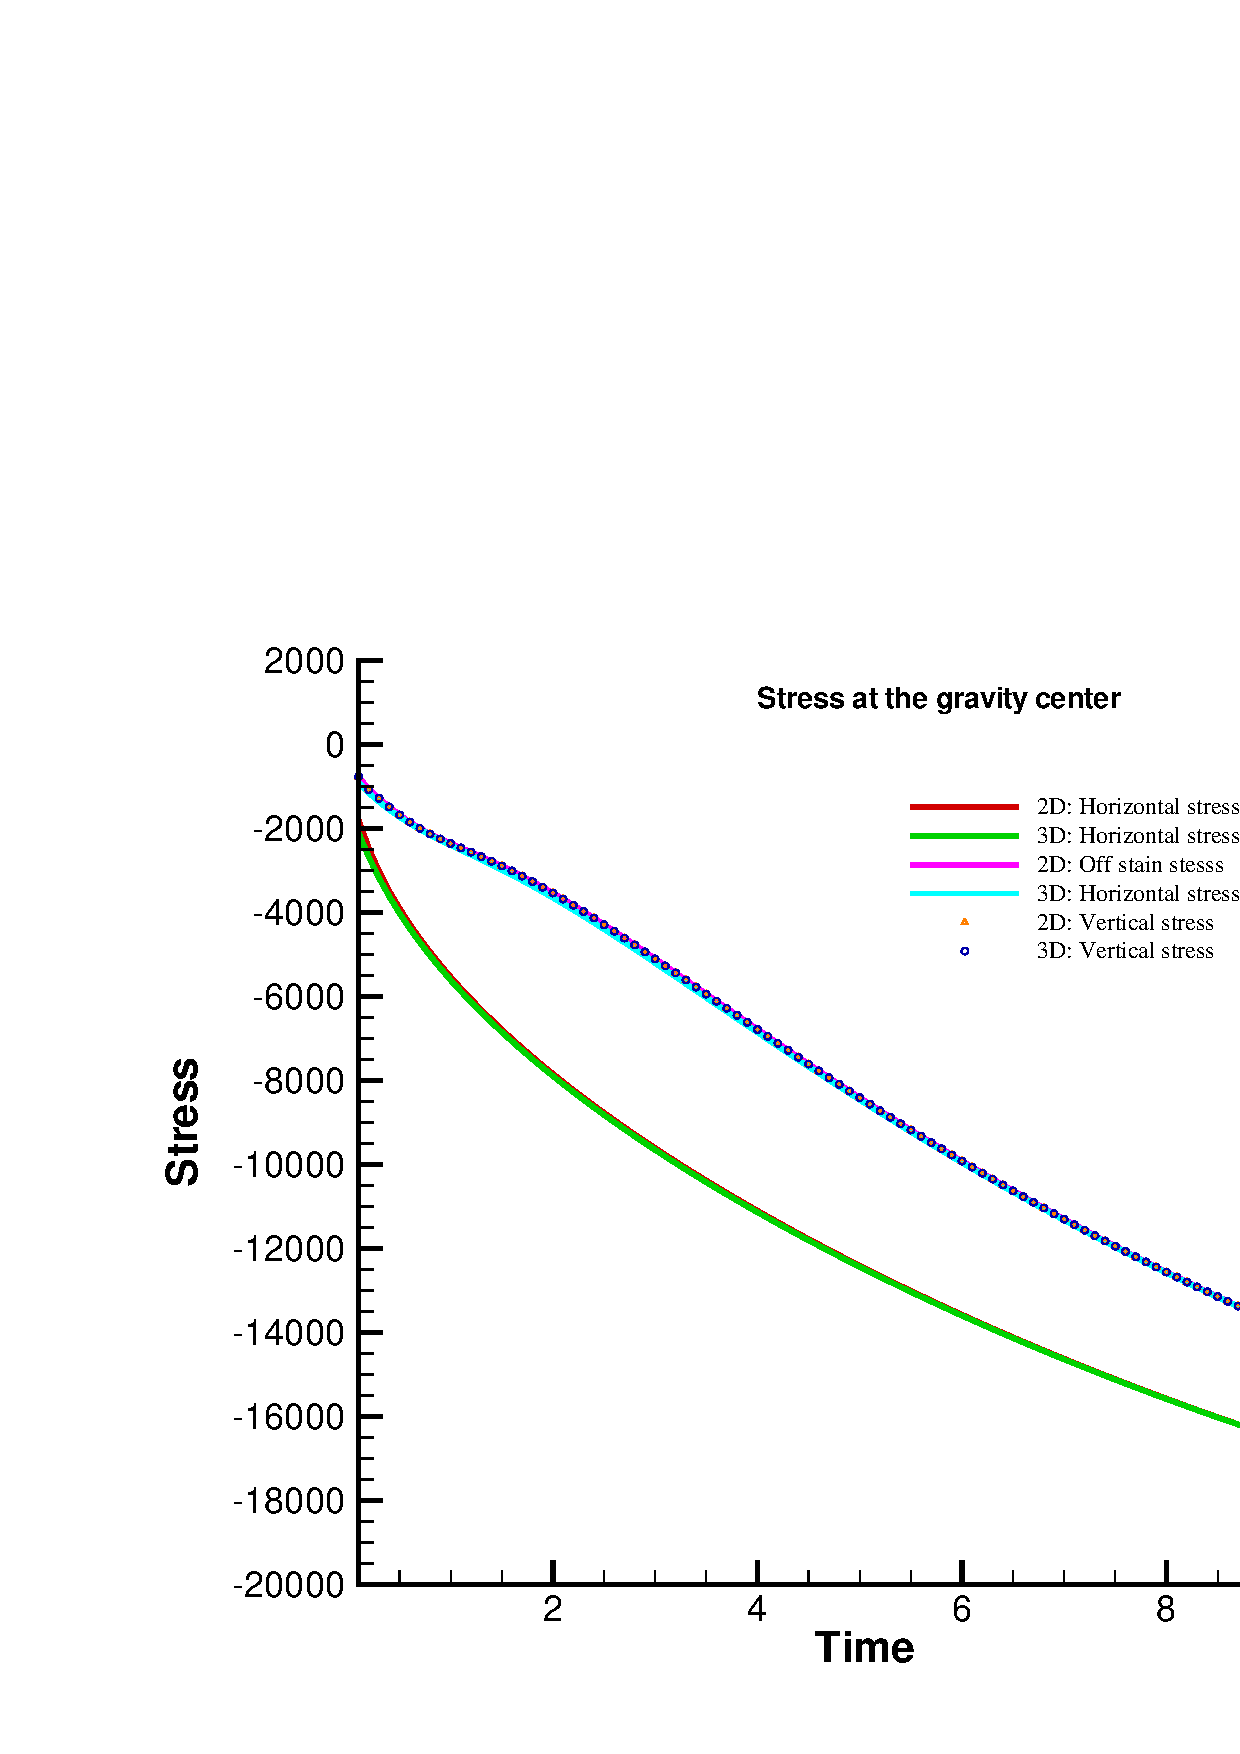
\includegraphics[height=7cm]{PART_III/TM/figures/2D_3D_cmp}\\
\caption{Comparison of 2D, 3D results }
\label{fig:TMcmp}
\end{figure}

%\clearpage
\section{Thermoelastic stress analysis in homogeneous material (3~D)}
\subsection{Definition}
The top and the bottom of a solid body that consists of one homogeneous  material are heated. The aim of the calculation is to find out the isotropic state of stress that is reached after the whole solid is heated. 
%
Figure \ref{fig61} shows a sketch of the calculation area assuming a homogeneous solid, a constant temperature in the whole body at the beginning and a heating of the top and the bottom of the body about 10~K.
Linear elastic material behaviour, isotropic thermal expansion and no gravity effect are assumed.
%
The $xy$-plane is the horizontal plane. The height of the body is in $z$-direction. The dimensions of this 3~D-model are 10~m in all directions. 
As deformations in $x$- and $y$-direction are suppressed, the increasing temperature evokes stresses within the solid. 
The used parameters of the solid represent the material behaviour of concrete (Table \ref{tab61}).

\begin{figure}[htbp]
\centering
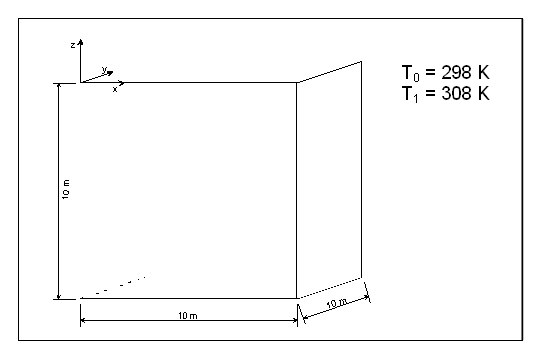
\includegraphics[width=0.6\textwidth]{PART_III/TM/figures/fig61}
\caption{Calculation area with one material}
\label{fig61}
\end{figure}

\begin{table}[htbp]
\centering
\caption{Model parameters}
\label{tab61}
\begin{tabular}{llrr}
\toprule
Symbol & Parameter & Value & Unit \\
\midrule
$T_0$  & Initial temperature (before heating) & 298 & $K$ \\
$T_1$  & Temperature after heating & 308 & $K$ \\
$\rho$  & Density of the solid &  2200 & $kg \cdot m^{-3}$  \\			
$E$ & Young's modulus of the solid & 25 & $GPa$ \\
$\nu$ & Poisson ratio & 0.27 & $-$ \\
$\alpha$ & Linear thermal expansion & 6.0$\cdot$10$^{-6}$ & $K^{-1}$ \\
$c$      & Specific heat capacity & 1.0 & $J\cdot kg^{-1}\cdot K^{-1}$ \\
$\lambda$ & Thermal conductivity & 1.0 & $W\cdot m^{-1}\cdot K^{-1}$ \\
\bottomrule
\end{tabular}
\end{table}


\subsection{Solution}
\subsubsection{Analytical solution}
The analytical solution can be derived from the time independent equation \eqref{eq61} to \eqref{eq63} with the assumptions of no deformation and an isotropic thermal expansion:
\begin{eqnarray}
\varepsilon_i & \equiv & 0 \nonumber \\[1.5ex]
\sigma_x & = & \sigma_y\,=\,\sigma_z\,=\,
-\frac{\alpha\cdot\Delta T\cdot E}{1-2\cdot\nu}
\label{eq64}
\end{eqnarray}
Equation \eqref{eq64} provides the stresses after heating the solid and shows an isotropic state of stress.

\subsubsection{Numerical solution}
The dimensions of this 3~D-model are 10~m in all directions. Deformations perpendicular to the outer surfaces are suppressed. The initial temperature in the whole area is 298~K. At the top and at the bottom of the model thermal boundary conditions are set with a temperature of 308~K. Thereby the heating of the solid about 10~K is simulated. 1000 hexahedral elements and 1331 nodes are used. The calculation is divided in 384 time steps with a constant time step length of 900 seconds. That means the heating of the solid within 4 days is simulated. The calculation model is sketched in Figure \ref{fig62}.


\begin{figure}[htbp]
\centering
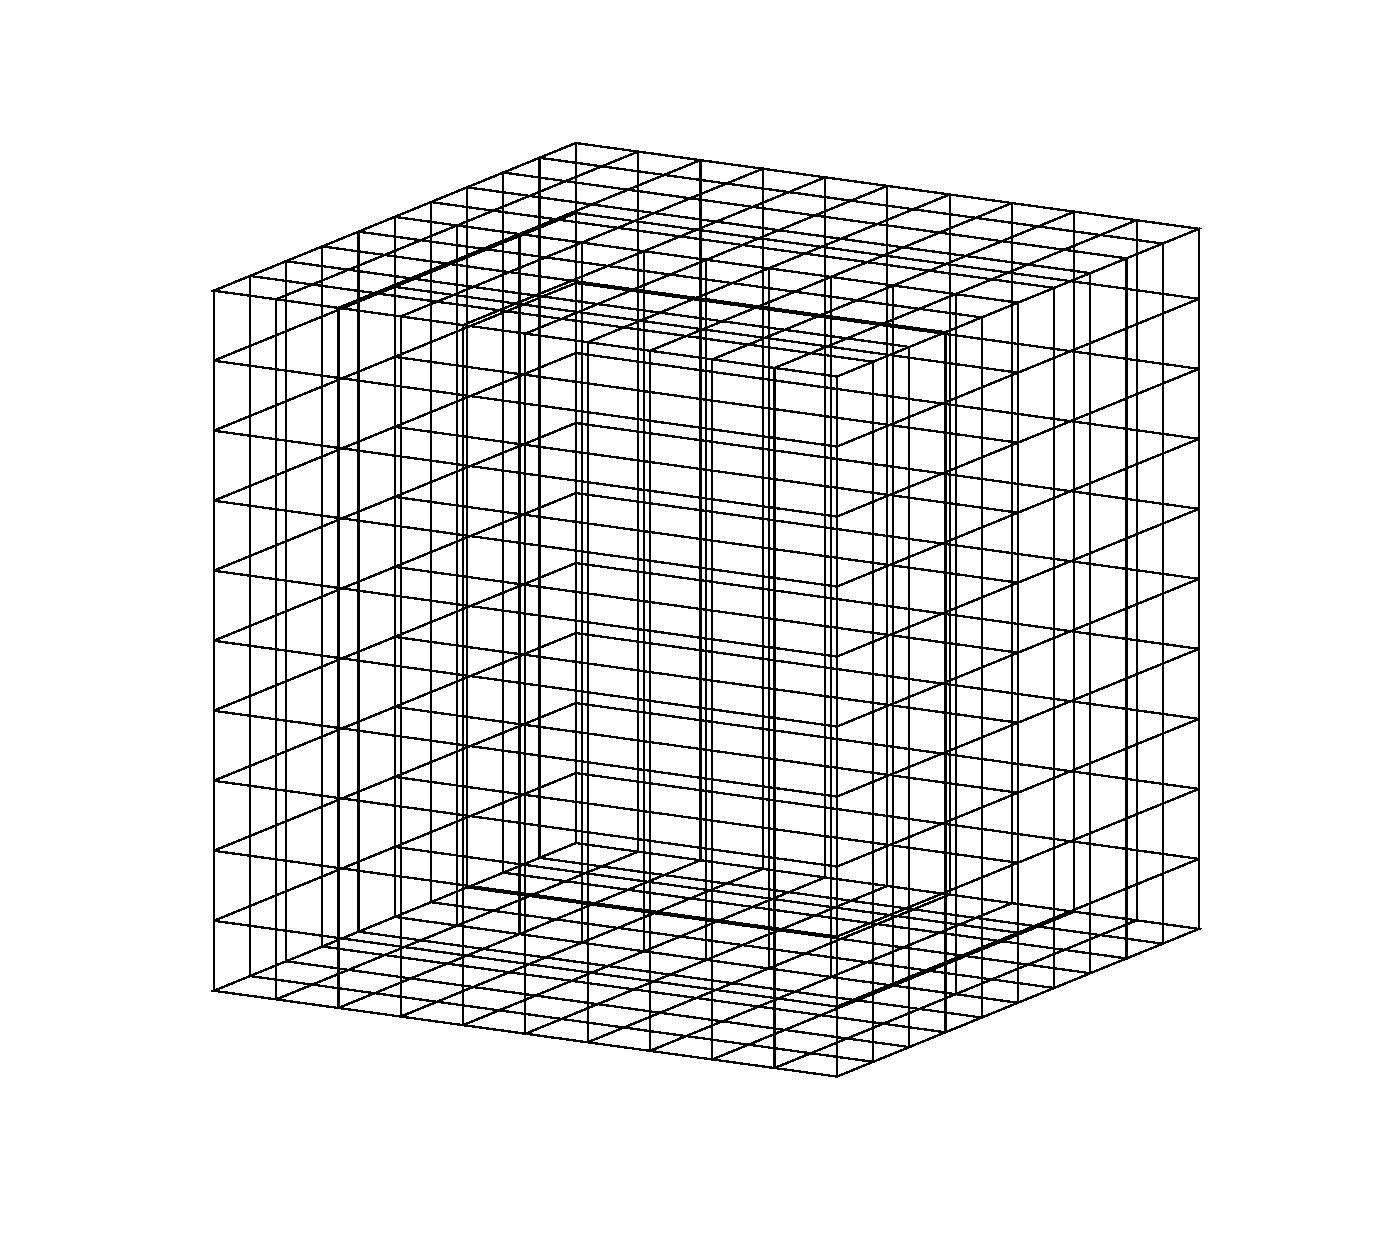
\includegraphics[width=0.6\textwidth]{PART_III/TM/figures/fig62}
\caption{Mesh for TM coupling homogeneous material 3D model}
\label{fig62}
\end{figure}

\subsection{Results}
With the analytical solution in equation \eqref{eq64} and the used parameters the stress values in the solid amount. This isotropic state of stress is reached after the whole solid is heated. The temporal development of the stresses in the centre of the model (at node 665) calculated is presented in Figure \ref{fig63}. The results of the 3~D simulation show an exact agreement with the analytical solutions.

\begin{figure}[htbp]
\centering
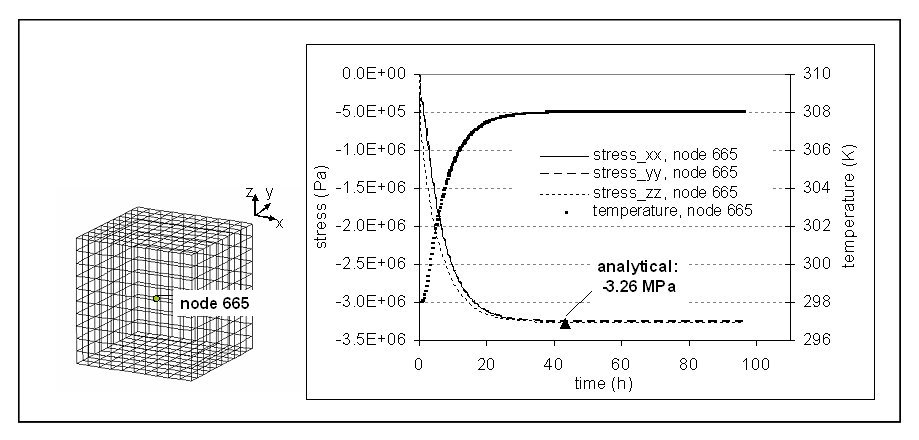
\includegraphics[width=0.9\textwidth]{PART_III/TM/figures/fig63}
\caption{Temporal stress development in the centre of the calculation model (node 665)}
\label{fig63}
\end{figure}


%\clearpage
\section{Thermoelastic stress analysis in composite materials (3~D)}
\subsection{Definition}
If there are two materials with different thermal expansions, the volume changes of the materials will be uncommon. The material with the higher thermal expansion expands more than the material with the low thermal expansion. If deformations at the outer boundaries are prevented, different states of stress will occur in these two materials. But the stresses perpendicular to the parting plane must be equal. The values of the stresses as a result of temperature changes can also easily be calculated by the Hooke's linear elastic model. The aim of this simulation is to specify the stresses at several areas in the solid. Figure \ref{fig64} shows a sketch of the calculation area. The model parameters are given in Table \ref{tab62}.

\begin{figure}[htbp]
\centering
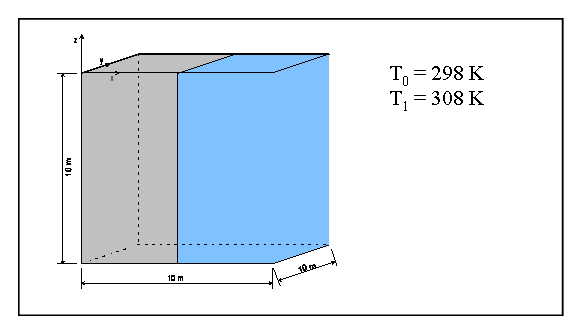
\includegraphics[width=0.6\textwidth]{PART_III/TM/figures/fig64}
\caption{Calculation area with two different materials}
\label{fig64}
\end{figure}

\begin{table}[htbp]
\centering
\caption{Model parameters}
\label{tab62}
\begin{tabular}{llrr}
\toprule
Symbol & Parameter & Value & Unit \\
\midrule
$T_0$  & Initial temperature (before heating) & 298 & $K$ \\
$T_1$  & Temperature after heating & 308 & $K$ \\
$\rho$  & Density of the solid &  2200 & $kg\cdot m^{-3}$  \\			
$E$ & Young's modulus of the solid & 25 & $GPa$ \\
$\nu$ & Poisson ratio & 0.27 & $-$ \\
$\alpha_1$ & Linear thermal expansion of material 1 & 6.0$\cdot$10$^{-6}$ & $K^{-1}$ \\
$\alpha_2$ & Linear thermal expansion of material 2 & 1.2$\cdot$10$^{-5}$ & $K^{-1}$ \\
$c$      & Specific heat capacity & 1.0 & $J\cdot kg^{-1}\cdot K^{-1}$ \\
$\lambda$ & Thermal conductivity & 1.0 & $W\cdot m^{-1}\cdot K^{-1}$ \\
\bottomrule
\end{tabular}
\end{table}

%\newpage

\subsection{Solution}
\subsubsection{Analytical solution}
The equations of the mechanical behaviour base on the Hooke's law for linear elastic materials (see equations \eqref{eq61} to \eqref{eq63}). The analytical solution can be derived from these time independent equations with the assumptions of suppressed deformations in $y$- and $z$-direction and an isotropic thermal expansion:
\begin{displaymath}
\varepsilon_x\,=\,\varepsilon_z\,\equiv\,0
\end{displaymath}
Additionally the stresses in x-direction (perpendicular to the parting plane between the two materials) must be equal:
\begin{displaymath}
\sigma_{x1}\,=\,\sigma_{x2}
\end{displaymath}
where indices denote different materials. 
Further the expansion of the one material leads to a compression of the other material with the same value in x-direction:
\begin{displaymath}
\varepsilon_{x1}\,=\,-\varepsilon_{x2}
\end{displaymath}
With these limiting conditions the analytical solutions are:
\begin{eqnarray}
\varepsilon_{x1} & = &
\frac{\Delta T}{2}\cdot\left(\alpha_1-\alpha_2\right)\cdot
\left(\frac{1+\nu}{1-\nu}\right)
\label{eq65} \\[1.5ex]
\varepsilon_{x2} & = & -\varepsilon_{x1}\,=\,
-\frac{\Delta T}{2}\cdot\left(\alpha_1-\alpha_2\right)\cdot
\left(\frac{1+\nu}{1-\nu}\right)
\label{eq66} \\[1.5ex]
\sigma_{x1} & = & \sigma_{x2}\,=\, E\cdot
\frac{\varepsilon_{x2}\cdot\left(1-\nu\right)-\alpha_2\cdot\Delta T\cdot\left(1+\nu\right)}{1-\nu-2\nu^2}
\label{eq67} \\[1.5ex]
\sigma_{y1} & = & \sigma_{z1}\,=\,
\frac{\nu\cdot\sigma_{x1}-\alpha_1\cdot\Delta T\cdot E}{1-\nu}
\label{eq68} \\[1.5ex]
\sigma_{y2} & = & \sigma_{z2}\,=\,
\frac{\nu\cdot\sigma_{x2}-\alpha_2\cdot\Delta T\cdot E}{1-\nu}
\label{eq69}
\end{eqnarray}
%{\small
%indices:
%
%\begin{tabbing}
%\=xxxx  \=xxxxxxxxxxxxxxxxxxxxxxx \kill
%\> 1 -- \> material 1 \\[1.0ex]
%\> 2 -- \> material 2
%\end{tabbing}
%}

Equations \eqref{eq65} to \eqref{eq69} provide the strains and stresses after heating the body of two materials. The state of stress is anisotropic.


\subsubsection{Numerical solution}
The calculation was done with a 3~D model. The $xy$-plane is the horizontal plane. The height of the body is in $z$-direction. The dimensions of this 3~D model are 10~m in all directions. The model includes 1000 hexahedral elements and 1331 nodes. Deformations perpendicular to the outer surfaces are suppressed. 
%Deformations in $x$- and $z$-direction are suppressed. 
The initial temperature in the whole area is 298~K. At the top and at the bottom of the model thermal boundary conditions are set with a temperature of 308~K. Thereby the heating of the body about 10~K is simulated. The used parameters of the solids represent the material behaviour of concrete. The calculation is divided in 1000 time steps with a constant time step length of 0.5 seconds. A sketch of the calculation model is shown in Figure \ref{fig65}.

\begin{figure}[htbp]
\centering
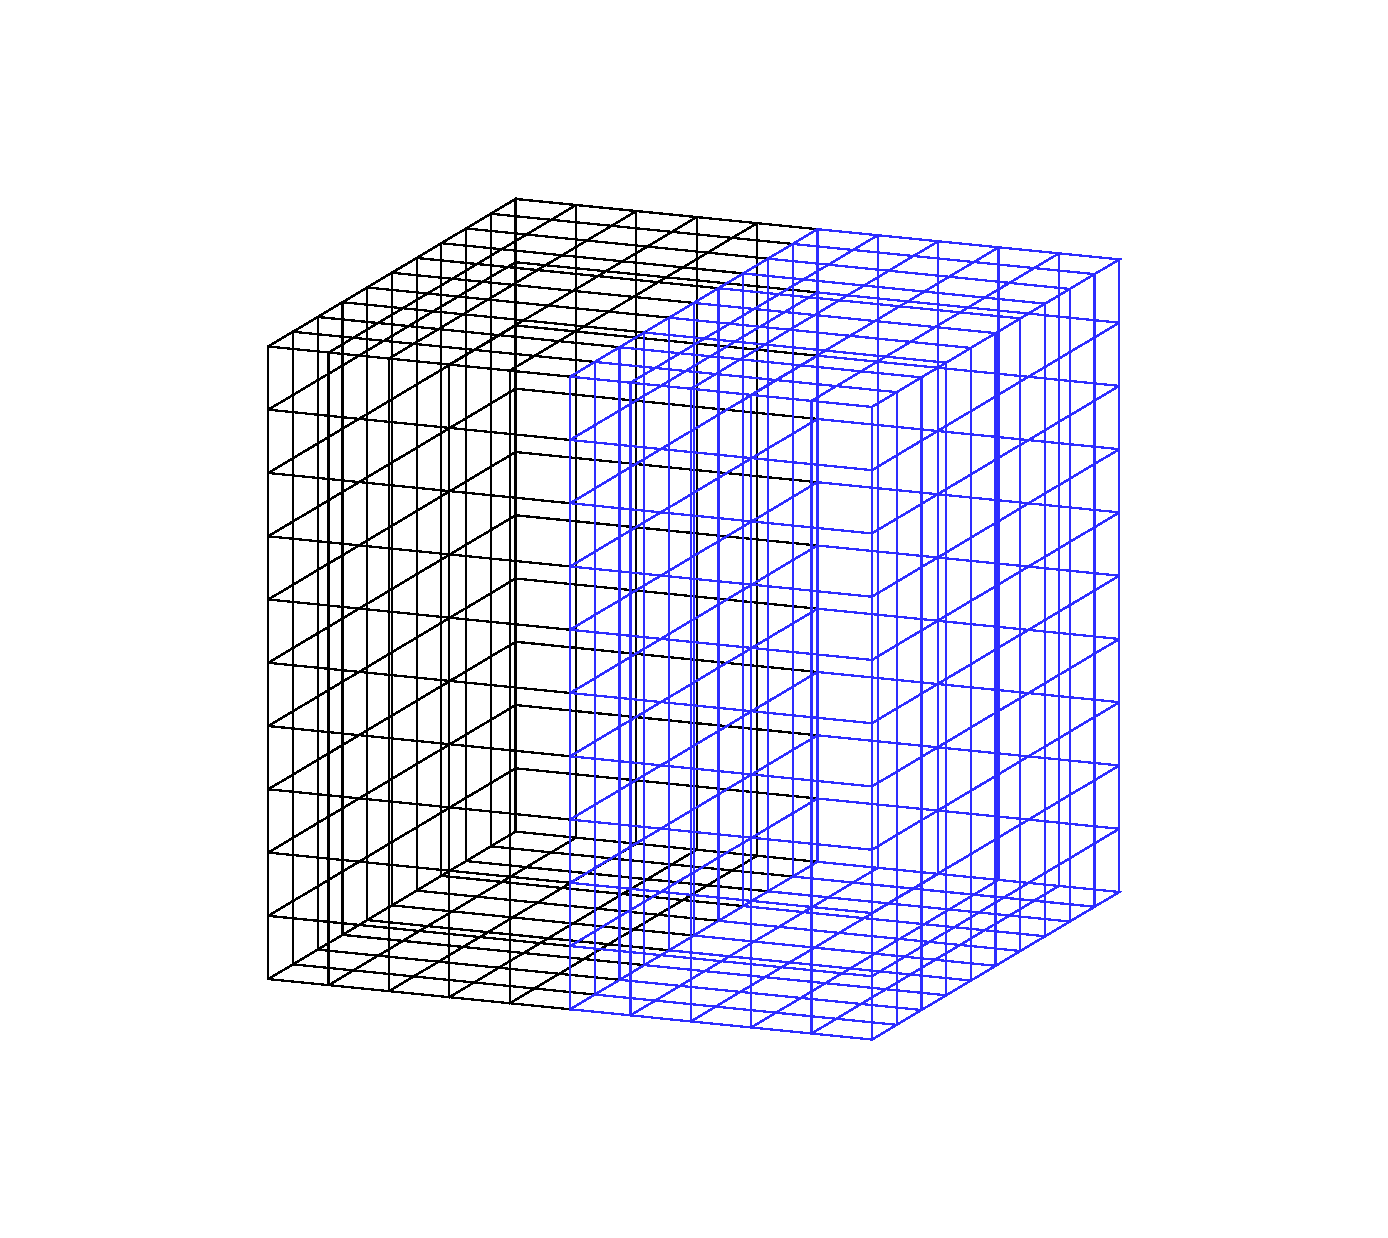
\includegraphics[width=0.6\textwidth]{PART_III/TM/figures/fig65}
\caption{Mesh for TM coupling 3D model with 2 materials}
\label{fig65}
\end{figure}



\subsection{Results}

With the analytical solution in equations \eqref{eq65} to \eqref{eq69} and the used parameters the values of the strains in $x$-direction at the parting plane amount
\begin{eqnarray*}
\varepsilon_{x1} & = & -5.219178\cdot 10^{-5} \\[1.5ex]
\varepsilon_{x2} & = & \phantom{-}5.219178\cdot 10^{-5}
\end{eqnarray*}
The values of the stresses are
\begin{eqnarray*}
\sigma_{x1} & = & \sigma_{x2}\,=\,-4891304.34\,\mathrm{Pa}
                             \,=\,-4.8913\,\mathrm{MPa} \\[1.5ex]
\sigma_{y1} & = & \sigma_{z1}\,=\,-3863907.08\,\mathrm{Pa}
                             \,=\,-3.8639\,\mathrm{MPa} \\[1.5ex]
\sigma_{y2} & = & \sigma_{z2}\,=\,-5918701.60\,\mathrm{Pa}
                             \,=\,-5.9187\,\mathrm{MPa}
\end{eqnarray*}
This anisotropic state of stress is reached after the whole body is heated. The temporal stress developments in several nodes calculated with both RockFlow and OGS are presented in Figure \ref{fig66} and Figure \ref{fig67}.
The results of the 3D simulation show an exact agreement with the analytical solutions.

\begin{figure}[!htbp]
\centering
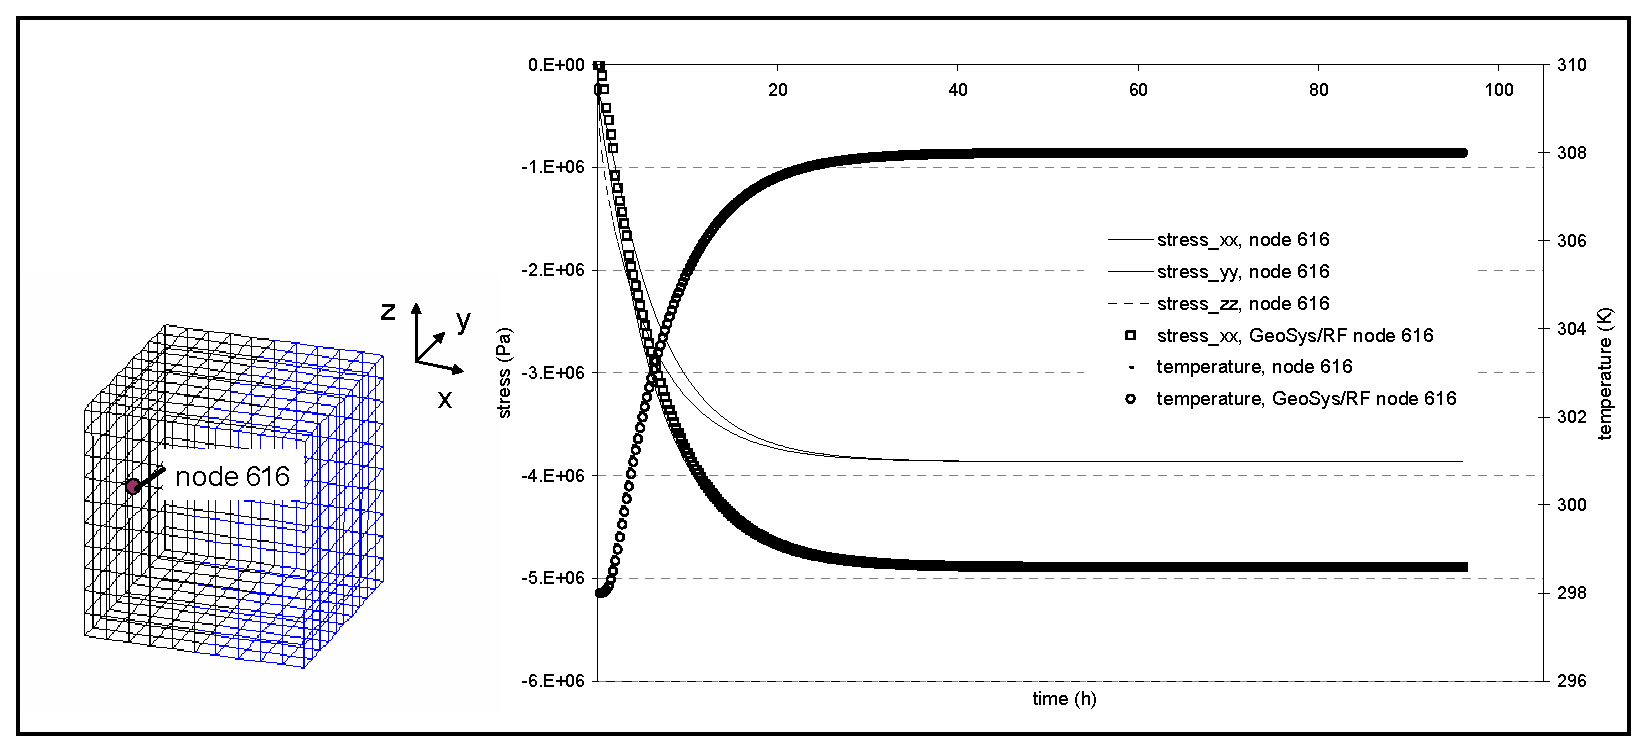
\includegraphics[width=125mm]{PART_III/TM/figures/fig66}
\caption{Temporal stress development in node 616}
\label{fig66}
\end{figure}

\begin{figure}[!htbp]
\centering
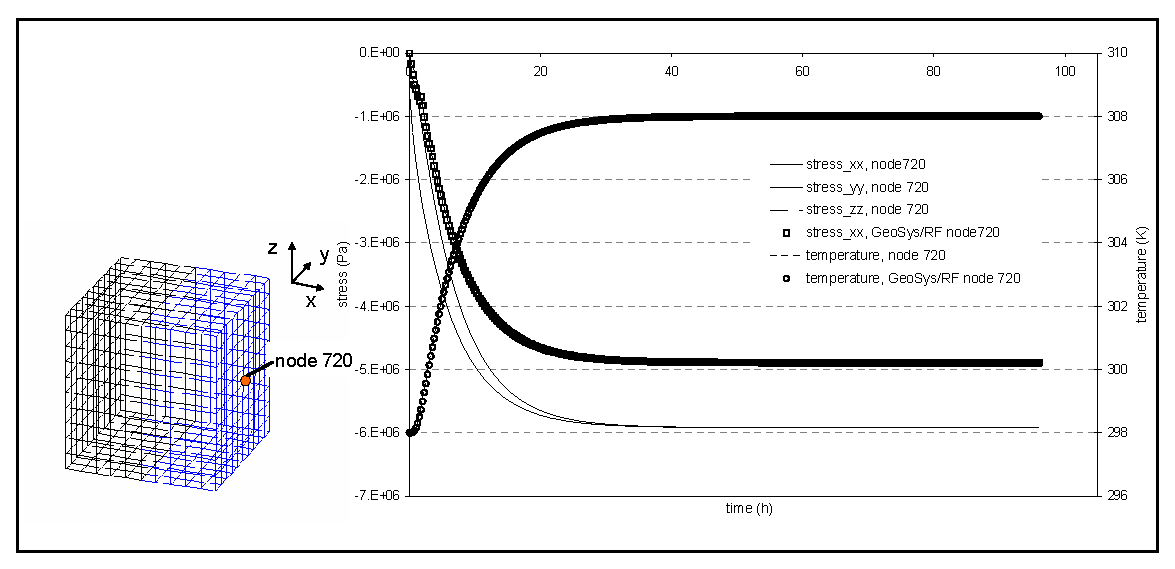
\includegraphics[width=125mm]{PART_III/TM/figures/fig67}
\caption{Temporal stress development in node 720}
\label{fig67}
\end{figure}



%\clearpage
\section{Thermoelastic deformation in a hollow cylinder}
\subsection{Definition}

A hollow cylinder which consists of a solid of a constant temperature is exposed to a higher temperature at the surface of its hole. As a result of the increased temperature the cylinder is expanding. The aim of this calculation is to get out the radial displacement as well as the temperature distribution that are caused by the thermal expansion process by the use of an axisymmetric model. 
Figure \ref{fig68} shows a sketch of the calculation area assuming a homogeneous solid, a constant temperature in the whole body at the beginning and a heating of the cylinder at the inner surface.
Linear elastic material behaviour and isotropic thermal expansion are assumed. Deformations in $y$-direction at the bottom and the top and in $x$-direction at the right border are suppressed. The used parameters of the solid are listed in Table \ref{tab63}.

\begin{figure}[htbp]
\centering
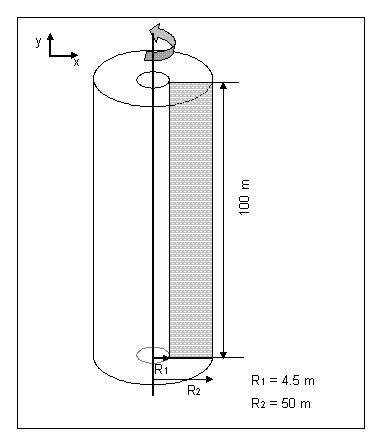
\includegraphics[width=0.45\textwidth]{PART_III/TM/figures/fig68}
\caption{Calculation area (grey area)}
\label{fig68}
\end{figure}

\begin{table}[htbp]
\centering
\caption{Model parameters}
\label{tab63}
\begin{tabular}{llrr}
\toprule
Symbol & Parameter & Value & Unit \\
\midrule
$T_0$  & Initial temperature (before heating) & 25 & $^{\circ}C$ \\
$q$  & Heat source & 30 & $W/m^2$ \\
$\rho$  & Density of the solid &  2000 & $kg \cdot m^{-3}$  \\			
$E$ & Young's modulus of the solid & 2.5 & $GPa$ \\
$\nu$ & Poisson ratio & 0.25 & $-$ \\
$\alpha$ & Thermal expansion & 4.2$\cdot$10$^{-5}$ & $K^{-1}$ \\
$\lambda$ & Thermal conductivity & 5.5 & $W\cdot m^{-1}\cdot K^{-1}$ \\
\bottomrule
\end{tabular}
\end{table}


%\textsl{Assumptions}
%
%\begin{tabbing}
%\=xxxxxxxxxxxx  \=xxxxxxxxxxxxxxxxxxxxxxx \kill
%\> Temperature: \> constant temperature in the whole body at the beginning, heating \\
%\> \> of the cylinder at the inner surface \\[1.0ex]
%\> Solid: \> homogeneous, finite dimensions, no deformation in $y$-direction at \\
%\> \> the bottom and the top, no deformation in $x$-direction at the right \\
%\> \> border, linear elastic material behaviour, isotropic thermal expansion
%\end{tabbing}

\subsection{Solution}
\subsubsection{Analytical solution} % WW derived the solution
For the hollow cylinder with the inner radius $R1$ and the outer radius $R2$ the following analytical solution for radial displacement $u_r$, stress $\sigma_r$ and temperature in dependency on the radius was used.% (Wang II, 2007).
\begin{eqnarray}
u_r & = &
\frac{q\,R_1\,\beta}{2\,\psi\,\kappa}\cdot r\cdot
\left(\ln\,r-\frac{1}{2}\right)\,+\,
\frac{A_0}{2}\,r\,+\,
\frac{A_1}{r}
\label{eq610} \\[2.0ex]
\sigma_r & = &
\psi\left[
-\frac{q\,R_1\,\beta}{2\,\psi\,\kappa}\cdot r\cdot
\left(\ln\,r+\frac{1}{2}\right)\,+\,
\frac{A_0}{2}\,-\,
\frac{A_1}{r^2}
\right] \nonumber \\[1.5ex]
 & & +\,
\lambda\left[
-\frac{q\,R_1\,\beta}{2\,\psi\,\kappa}\cdot r\cdot
\left(\ln\,r-\frac{1}{2}\right)\,+\,
\frac{A_0}{2}\,+\,
\frac{A_1}{r^2}
\right] \nonumber \\[1.5ex]
& & -\,\beta\left[
\frac{R_1\,q}{\kappa}\,\ln\left(\frac{R_2}{r}\right)\,+\,T_0
\right]
\label{eq611} \\[2.0ex]
T(r) & = &
\frac{R_1\,q}{\kappa}\,\ln\left(\frac{R_2}{r}\right)\,+\,T_0
\label{eq612}
\end{eqnarray}
{\small
where
\begin{displaymath}
\psi\,=\,\lambda\,+\,2\,G\qquad\mathrm{and}\qquad
\beta\,=\,\alpha\left(3\,\lambda\,+\,2\,G\right)
\end{displaymath}
with
\begin{tabbing}
\=xxxxxx \=xxxxxxxxxxxxxxxxxxxxxxxxxxxxxxxxx  \kill
\> $\lambda$   \> -- Lam$\acute{\mathrm{e}}$ elastic constant \\[0.5ex]
\> $G$         \> -- shear modulus \\[0.5ex]
\> $\alpha$    \> -- thermal expansion coefficient \\[0.5ex]
\> $\kappa$    \> -- thermal conductivity \\[0.5ex]
\> $A_0,\,A_1$ \> -- integration constants
\end{tabbing}
}

At the outer surface of the hollow cylinder (where $r=R_2$) there is no deformation, that means the displacement $u_{R2}$ is zero. Therefore equation \eqref{eq610} is set equal to zero for this boundary and adapted to $A_0$.
\begin{equation}
A_0\,=\,-\frac{2\,A_1}{R^2_2}\,-\,2\cdot B\cdot
\left(\ln\,R_2\,-\,\frac{1}{2}\right)
\label{eq613}
\end{equation}
{\small
where
}
\begin{displaymath}
B\,=\,\frac{q\,R_1\,\beta}{2\,\psi\,\kappa}
\end{displaymath}

At the inner surface of the hollow cylinder (where $r=R_1$) no stress is effected by the expansion because this boundary is phreatic. Therefore equation \eqref{eq611} is set equal to zero and $A_1$ is calculated by using equation \eqref{eq614}.
{\small
\begin{equation}
A_1=
\frac{
 \beta\!\left(\frac{
 \textstyle{R_1\,q}}{\textstyle{\kappa}}
 \ln\!\left(\frac{\textstyle{R_2}}{\textstyle{r}}\right)+T_0\right)
 \!+\!
 \lambda B\!\left(\ln R_1\!-\!\frac{1}{2}\right)\!+\!
 \psi B\!\left(\ln R_1\!+\!\frac{1}{2}\right)\!-\!
 \left(\frac{\textstyle{\lambda\!+\!\psi}}{\textstyle{2}}\right)
 2B\left(\ln R_2\!-\!\frac{1}{2}\right)
}
{\frac{
 \textstyle{\lambda-\psi}}{\textstyle{R^2_1}}-
 \frac{\textstyle{\lambda+\psi}}{\textstyle{2}}\cdot
 \frac{\textstyle{2}}{\textstyle{R^2_1}}\cdot
}
\label{eq614}
\end{equation}
}
After having solved this equation, $A_1$ is used to calculate $A_0$.




\subsubsection{Numerical solution}
The axisymmetric model is in the $xy$-plane. The inner radius $R1$ of the cylindrical model is 4.5~m and the outer radius $R2$ 50~m. The cylinder is 100~m high. The initial temperature in the whole area is 25$^{\circ}$C. As boundary condition deformations in $y$-direction at the bottom and the top are suppressed, as well as deformations in $x$-direction at the right border. At the right boundary of the model a thermal boundary condition is set with a constant value of 25$^{\circ}$C. At the left boundary a source term for heat flux of $q=30$~W/m$^2$ is defined. Thereby the continuous heating of the solid is simulated.  The simulation of only one time step is done. The numerical model consists of 766 triangular elements and 426 nodes as sketched in Figure \ref{fig69}.

\begin{figure}[htbp]
\centering
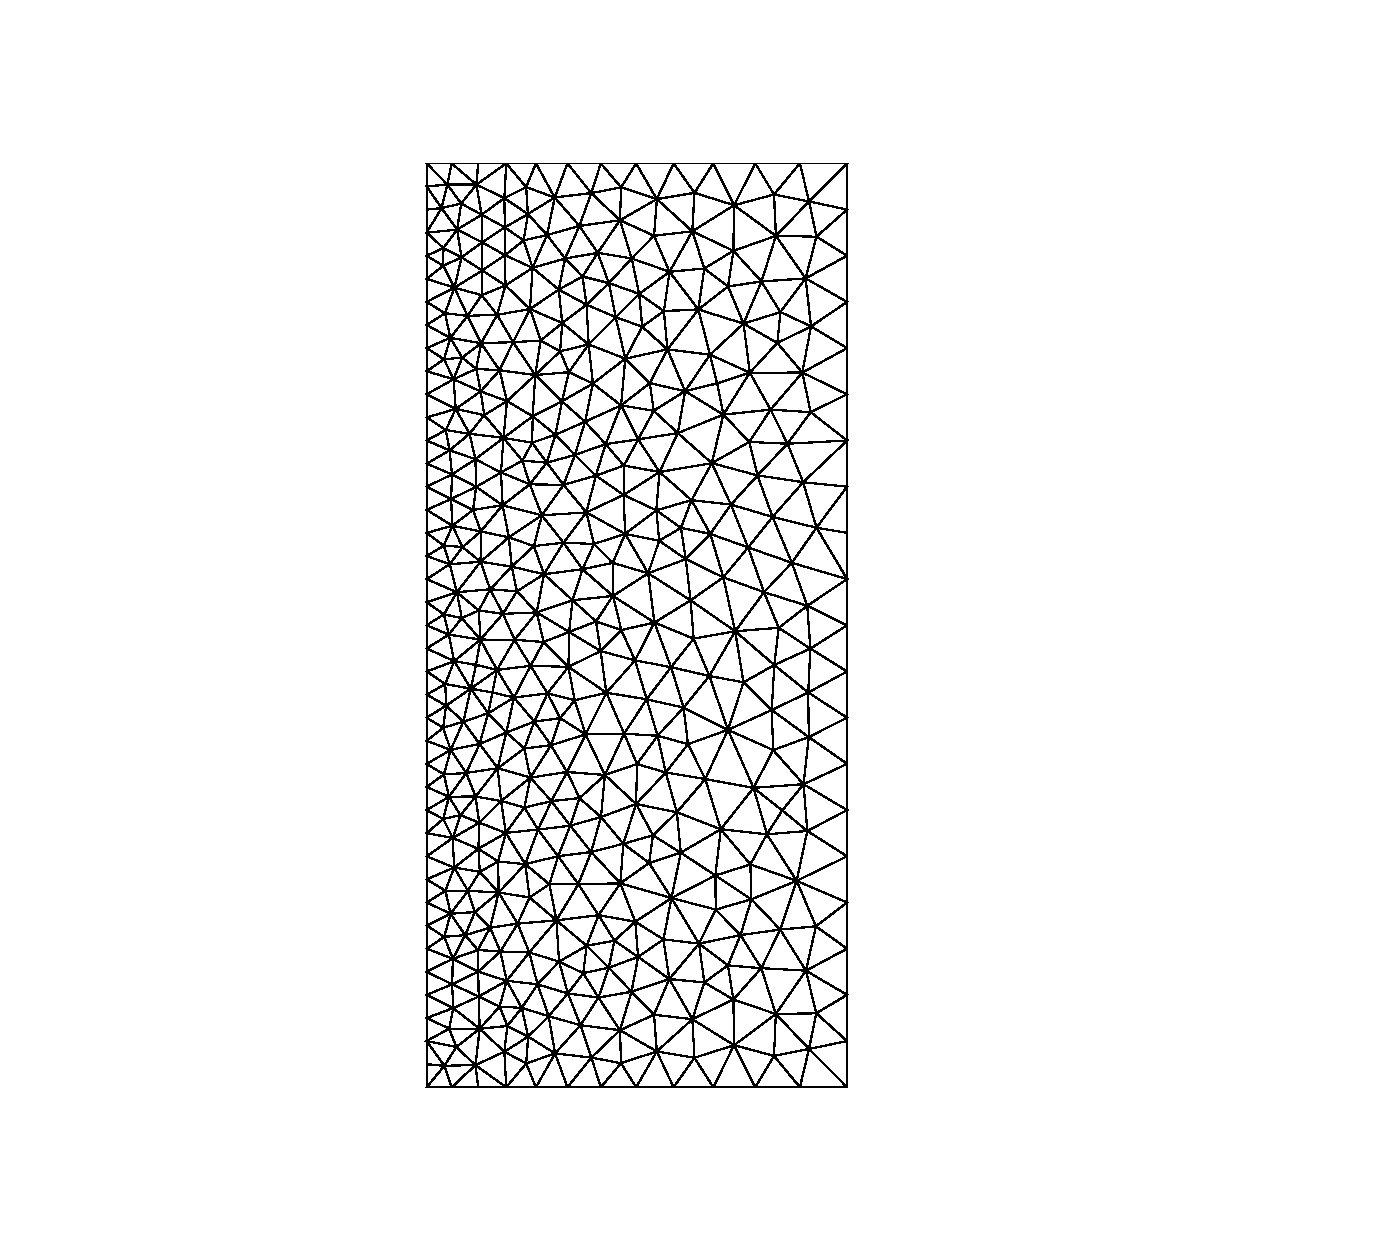
\includegraphics[width=0.6\textwidth]{PART_III/TM/figures/fig69.eps}
\caption{Mesh for TM coupling hollow cylinder model (2D axisymmetric)}
\label{fig69}
\end{figure}

\begin{figure}[htbp]
\centering
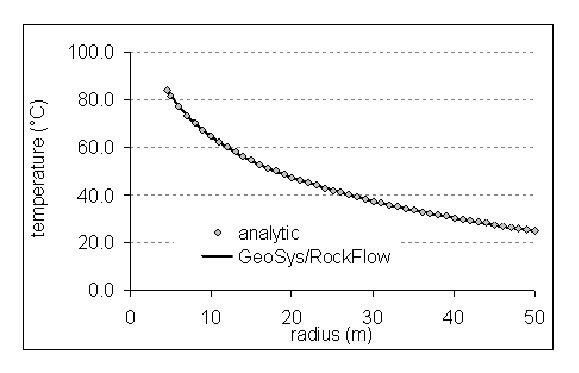
\includegraphics[width=0.7\textwidth]{PART_III/TM/figures/fig610}
\caption{Temperature distribution over the radius}
\label{fig610}
\end{figure}

\begin{figure}[htbp]
\centering
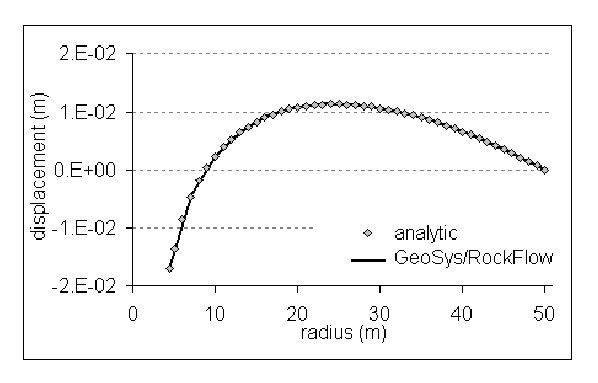
\includegraphics[width=0.7\textwidth]{PART_III/TM/figures/fig611}
\caption{Displacements in radial direction}
\label{fig611}
\end{figure}

\begin{figure}[htbp]
\centering
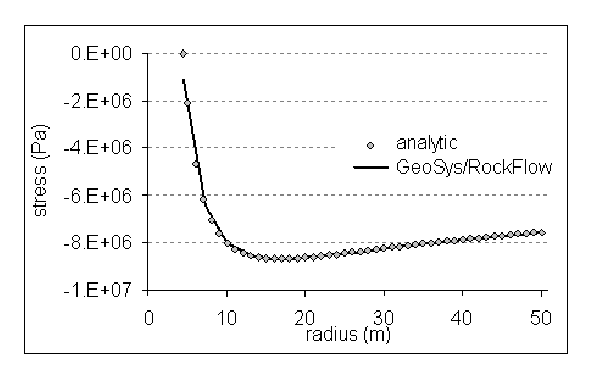
\includegraphics[width=0.7\textwidth]{PART_III/TM/figures/fig612}
\caption{Stresses in radial direction}
\label{fig612}
\end{figure}

\subsection{Results}
The results of the analytical equations for stresses, displacements and temperatures are compared to those of the numerical simulation by OGS. 
With the equations \eqref{eq614} and \eqref{eq613} and the used parameters, the integration constants in the analytical solution are obtained as: 
\begin{eqnarray*}
A_0 & = & \phantom{-}5.96\cdot10^{-3} \\[1.0ex]
A_1 & = & -1.19\cdot10^{-1}
\end{eqnarray*}

Figure \ref{fig610} shows the temperature distribution over the radius of the hollow cylinder. In Figure \ref{fig611} displacements in radial direction that are caused by the thermal expansion are depicted. In addition you can find the induced stresses in Figure \ref{fig612}. Obviously, with the axisymmetric model a OGS simulation generates comprehensible results that meet well the analytic solution.
